%\documentclass[10pt,a4paper,twoside]{article}
\documentclass[10pt,a4paper]{article}
\usepackage[utf8]{inputenc}
\usepackage[german]{babel}
\usepackage{amsmath}
\usepackage{amsfonts}
\usepackage{amssymb}
\usepackage{units} % soll ich das verwenden? oder siunitxs oder garnix?
\usepackage{hyperref}
\hypersetup{
%    bookmarks=true,
    pdftoolbar=true,
    pdfmenubar=true,
    pdffitwindow=false,
    pdfstartview={FitH},
    pdftitle={HVDC},		% XXX: fix
    pdfauthor={Michael F. Sch\"onitzer},
    pdfsubject={HVDC},	% XXX: fix
    pdfkeywords={HVDC} {Strom} {Physik},	% XXX: fix
    pdfnewwindow=true,
    colorlinks=true,
    linkcolor=black,
    citecolor=black,
    filecolor=black,
    urlcolor=blue
}
\newcommand{\degree}{$^\circ$}
\newcommand{\q}{\glqq }
\newcommand{\qe}{\grqq }
\newcommand{\rot}{\mathrm{rot\:}}

\usepackage{rotating}
\usepackage[basic]{circ}


\author{Michael F. Schönitzer}
\title{HGÜ}
\begin{document}
\maketitle

\section{Geschichtliches}

\section{Gleichstrom}
Die Energieübertragung mittels Gleichstrom ist im Grunde relativ einfach und bereits aus der Schule bekannt, wir wollen sie daher hier nur kurz zusammenfassen.
Eine Gleichspannungsquelle liefert einen zeitlich konstanten Potentialunterschied, elektrische Spannung $U$ genannt. Legt man an diese einen ohmschen Widerstand $R$ an, so fließt durch ihn eine zeitlich konstanter Strom
\begin{equation}
I = \frac{U}{R}
\end{equation}
Und leistet an ihm die Leistung
\begin{equation}
P = U \cdot I
\end{equation}



\section{Einphasen-Wechselstrom}\label{wechsel}
Beim Einphasen-Wechselstrom hat man einen Nullleiter und einen Leiter auf der eine sinusförmige Wechselspannung mit der Amplitude $U_0$ anliegt:
\begin{equation}
U(t)=U_0 \cdot \cos(\omega t + \varphi)
\end{equation}
Dieser Leiter wird in der Elektrotechnik oft umgangssprachlich als Phase bezeichnet, wir wollen davon hier jedoch nicht Gebrauch machen, da wir physikalisch korrekter den Faktor $\varphi$ als Phasenverschiebung oder kurz Phase bezeichnen werden.

Legt man obige Spannung an einem ohmschen Widerstand R an, so fließt durch ihn der Strom $I(t)= \frac{U(t)}{R} = I_0 \cdot \cos(\omega t + \varphi)$ mit $I_0 = U_0/R$.
Die elektrische Leistung $P$ die an dem Widerstand geleistet wird, wird analog zur Gleichspannungstechnik als Produkt Produkt aus Spannung und Strom definiert, dabei beziehen sich jedoch alle drei Größen auf die momentanen Werte:
\begin{equation}
P(t) = U(t) \cdot I(t) \stackrel{\mathrm{\varphi=0}}= U_0 I_0 \cdot \cos^2(\omega t)
\end{equation}
Berechnen wir nun den Zeitlichen Mittelwert der Leistung
\begin{equation}\label{Wirkleistung_ohne_phi}
\bar{P}=\frac1T \int\limits_0^T dt\: U_0 I_0 \cos^2 \omega t = \frac12 U_0 I_0 \qquad\mathrm{mit}\; T=2\pi/\omega
\end{equation}
Vergleicht man dies mit der Leistung eines Gleichstroms $P=U\cdot I$, so sieht man, dass eine Gleichspannung mit $U=U_0 / \sqrt2$ und der daraus folgend Strom $I=I_0 / \sqrt2$ dieselbe Leistung erbringt.
Deshalb definiert man die Effektivspannung und den Effektivstrom eines Wechselstroms als:
\begin{equation*}
U_{\mathrm{eff}} = \frac{U_0}{\sqrt2} \qquad I_{\mathrm{eff}} = \frac{I_0}{\sqrt2} \qquad \bar{P}=U_{\mathrm{eff}}I_{\mathrm{eff}}
\end{equation*}
Im folgenden werden wir mit $U$ beziehungsweise $I$ die Effektivwerte, mit $U(t)$ beziehungsweise $I(t)$ die Momentanwerte und mit $U_0$ beziehungsweise $I_0$ die Amplituden bezeichnen.


%%% INCLUDE-FILE: Spulen_Kondensatoren.tex %%%

\subsection{Spulen und Kondensatoren im Wechselstromkreis}
Während sich Spulen und Kondensatoren in Gleichstromkreisen keine besondere Rolle spielen, sind ihre Auswirkungen auf den Stromfluss in einem Wechselstromkreis außerordentlich wichtig. Zur besseren Verständlichkeit betrachten wir beide zunächst getrennt und erst dann den allgemeinen Fall mit Spule, Kondensator und ohmschen Widerstand. Diese Kapitel richtet sich weitestgehend nach \cite{Demtroeder}.

\subsubsection{Spulen in Wechselstromkreisen}
Wir betrachten nun einen Wechselstromkreis mit vernachlässigbaren Widerständen, in welchem sich eine Spule befindet. Ein Stromfluss in der Spule führt zu einem Magnetfeld. Da der Stromfluss in der Spule jedoch ständig sein Vorzeichen ändert, wird abwechselnd ein Magnetfeld in die eine Richtung aufgebaut und nach seinem Zusammenbrechen dann ein Magnetfeld mit umgekehrter Ausrichtung aufgebaut.
Die Summe aller Spannungen muss in einem Stromkreis immer Null sein:
$ U_Q(t) + U_\mathrm{ind}(t) = 0 $,
wobei $U_Q$ die von der Quelle angelegte Spannung ist und $U_\mathrm{ind}$ die durch das Magnetfeld induzierte Spannung in der Spule ist. Letztere berechnet sich durch
\begin{equation}
U_\mathrm{ind}(t) = - L \cdot \frac{\mathrm dI(t)}{\mathrm dt}
\end{equation}
Daraus folgt durch Einsetzen und Integrieren
\begin{align}
%U_Q + U_{ind} =& 0 \nonumber \\
%\Rightarrow\;
U_0 \cos \omega t =& L \cdot \frac{\mathrm dI(t)}{\mathrm dt} \nonumber \\ 
\Rightarrow\; I(t) =& \frac{U_0}{L} \int \cos \omega t \mathrm dt = \nonumber \\ 
=& \frac{U_0}{\omega L} \sin \omega t = \nonumber\\
=& I_0 \sin \omega t \qquad mit\qquad I_0 = \frac{U_0}{\omega L}  \nonumber\\
=& I_0 \cos(\omega t - 90^\circ)
\end{align}
Es gibt also eine relative Phasenverschiebung zwischen dem Strom- und Spannungsverlauf: der Strom hinkt der Spannung also um \unit{90}{\degree} hinterher und wir definieren analog zum ohmschen Widerstand den Betrag des induktiven Widerstand als den Quotient zwischen $U_0$ und $I_0$:
\begin{equation}
\left|Z_L\right| = \frac{U_0}{I_0} = \omega \cdot L
\end{equation}
Dies wird auch Induktanz $X_L = \left|Z_L\right| = \omega \cdot L$ genannt.

\subsubsection{Kondensatoren im Wechselstromkreis}
Analog zur Spule können wir auch die Auswirkung eines Kondensators im Stromkreis berechnen.
Wir beginnen dabei mit der Gleichung
\begin{equation}
U(t) = \frac{Q(t)}{C}
\end{equation}
für den Kondensator und differenzieren diese nach der Zeit:
\begin{equation}
\frac{dU(t)}{dt} = \frac{1}{C}\frac{dQ(t)}{dt} = \frac{1}{C} \cdot I(t)
\end{equation}
Da die angelegte Spannung $U_Q$ der Spannung am Kondensator entspricht, gilt:
\begin{equation}
U_0\cdot \omega \sin \omega t = \frac{1}{C} \cdot I(t)
\end{equation}
und somit
\begin{equation}
I(t) = U_0\cdot \omega C \cdot\cos\left( \omega t + 90^\circ\right)
\end{equation}
Während bei einer Spule also der Strom der Spannung um \unit{90}{\degree} hinterher hinkt, eilt er bei einem Stromkreis mit Kondensator um \unit{90}{\degree} voraus. Wir ahnen bereits, dass diese beiden Effekte sich gegenseitig aufheben können.
Auch hier können wir analog zum ohmschen Widerstand den Betrag des kapazitiven Widerstands definieren:
\begin{equation}
\left|Z_C\right| = \frac{U_0}{I_0} = \frac{1}{\omega C}
\end{equation}
Der Begriff Kapazitanz bezeichnet $X_C = -\left|Z_C\right| = -\frac{1}{\omega C}$.

\subsubsection{Allgemeiner Fall}
Betrachten wir nun einen Wechselstromkreis mit einer Induktivität, einer Kapazität und einem ohmschen Widerstand. Wieder gilt die 2. Kirchhoffsche Regel $\sum U = 0$:
\begin{equation}
U_Q(t) = L \cdot \frac{\mathrm{d}I(t)}{\mathrm{d}t} + \frac{Q(t)}{C} + I(t) \cdot R
\end{equation}
Wir entledigen uns der unbekannten Ladung, indem wir nach der Zeit differenzieren:
\begin{equation}
\frac{\mathrm dU_Q(t)}{\mathrm dt} = L \cdot \frac{\mathrm{d^2}I(t)}{\mathrm{d}t^2} + \frac{I(t)}{C} + \frac{\mathrm dI(t)}{\mathrm dt} \cdot R
\end{equation}
Diese Differenzialgleichung können wir mithilfe eines komplexem e-Ansatzes lösen:
Wir lösen diese Differenzialgleichung im Komplexen und betrachten dann den Realteil der komplexen Lösung gemäß Superpositionsprinzip als die physikalisch sinnvolle Lösung. Unser Ansatz lautet:
\begin{equation}
U_Q(t) = U_0 e^{i\omega t},	\qquad	I(t) = I_0 e^{i(\omega t-\varphi)}
\end{equation}
Die Wahl von U als komplexe Exponentialfunktion ist deshalb möglich, da der Realteil der komplexen Exponentialfunktion die Kosinus-Funktion ist.
\begin{equation}
Re\left[ U_0 e^{(i\omega t)}\right]  = U_0 \cos{(\omega t)}
\end{equation}
Durch Einsetzen in den Ansatz erhalten wir:
\begin{equation}
i\omega U_Q(t) = (- L \omega^2 + i \omega R  + \frac{1}{C}) \cdot I(t)
\end{equation}
Wir definieren analog zum klassischen ohmschen Widerstand den komplexen Widerstand als Quotient von Spannung und Strom:
\begin{equation}
Z = \frac{U_Q(t)}{I(t)} = R + i ( \omega L - \frac{1}{\omega C})
\end{equation}
Wir stellen diese komplexe Größe nun in Polardarstellung
\begin{equation}
Z = |Z| \cdot e^{i\varphi}
\end{equation}
mit
\begin{equation}\label{eq:Zpolar}
|Z| = \sqrt{ R^2 + \left( \omega L - \frac{1}{\omega C} \right) }\quad {\mathrm{und}} \quad \tan\varphi = \frac{Im[Z]}{Re[Z]} = \frac{\omega L - \frac{1}{\omega C}}{R}
\end{equation}
dar. Kehren wir nun zur Betrachtung im Reellen zurück, um $I_0$ zu bestimmen:
\begin{align}
\nonumber
Re\left[ I \right]
&= Re\left[ \frac{U(t)}{Z} \right] =\\\nonumber
&= Re\left[ \frac{U_0 e^{i\omega t}}{|Z|\cdot e^{i\varphi}} \right] =\\\nonumber
&= \frac{U_0}{|Z|} Re\left[ e^{i(\omega t - \varphi)} \right] =\\
&= \frac{U_0}{|Z|} \cos(\omega t - \varphi) = I_0 \cos(\omega t - \varphi)
\end{align}

Der Tangens der Phasenverschiebung ist also der Quotient aus Imaginärteil und Realteil des komplexen Widerstands, während die Amplitude der Stromkurve die Amplitude der Spannung durch den Betrag des komplexen Widerstands ist.
Man erkennt in \eqref{eq:Zpolar} leicht, dass die Phasenverschiebung null ist, wenn der Imaginärteil null ist, was für 
\begin{equation}
\omega L = \frac{1}{\omega C}
\end{equation}
der Fall ist. Bei richtiger Wahl von Induktivitäten bzw. Kapazitäten kann man also die durch eine Kapazität bzw. Induktivität entstehende Phasenverschiebung zwischen Strom und Spannung auslöschen.



\subsection{Wirk-, Schein- und Blindleistung und der Leistungsfaktor}
Die Größen Spannung, Leistung und die Phasenverschiebung beschreiben das System vollständig, die Arbeit mit diesen Größen ist jedoch oft kompliziert und aufwändig. Daher zieht man häufig die Beschreibung mit den Größen Wirk-, Schein- und Blindleistung vor, weshalb wir diese hier definieren und näher betrachten wollen.

Die Wirkleistung ist diejenige Leitung welche real genutzt werden kann, sie wird manchmal auch als aktive Leistung oder Nutzleistung bezeichnet. Sie ist das arithmetische Mittel über die Augenblicksleistung:
\begin{equation}
P = \overline{p} = \overline{(t) \cdot I(t)}
\end{equation}
Für kosinusförmige Spannungs- und Stromverläufe wird daraus:
\begin{equation}
P = U_0 I_0 \cdot \frac{1}{2\pi} \int\limits_0^{2\pi} \cos\left( \omega t\right) \cos \left(\omega t - \varphi\right)
= \frac{1}{2} U_0 I_0 \cos \varphi
\end{equation}
Dies entspricht natürlich dem unter \ref{Wirkleistung_ohne_phi} berechneten, jedoch nun mit Phasenverschiebung. Mit den Effektivwerten wird daraus also:
\begin{equation}
P =  U_{\mathrm{eff}} I_{\mathrm{eff}} \cdot \cos \varphi
\end{equation}
Die Wirkleistung wird in Watt (1 W = 1 V$\cdot$A) gemessen.

Die Scheinleistung, ist hingegen das Produkt aus Spannung und Strom ohne Phasenfaktor. Die Verluste und die Beanspruchung der Komponenten verhält sich als würde eine scheinbare Wirkleistung dieser Größe übertragen werden. Sie stellt die bei einer gewissen Beanspruchung der Leitungskomponenten, die maximal übertragbare Wirkleistung dar. Sie ist deshalb immer größer oder gleich der Wirkleistung, wobei die Gleichheit für die Fall eintritt das die Phasenverschiebung null ist.
\begin{equation}
S = U_{\mathrm{eff}} I_{\mathrm{eff}} \geq P
\end{equation}
Die Scheinleistung ist zwar das Produkt aus Spannung (gemessen in Volt) und Strom (gemessen in Ampere), sie ist jedoch keine Leistung im physikalischen Sinn, deshalb wird sie nicht in Watt, sondern in Voltampere (VA) gemessen wird.

Als nächstes wollen wir den Leistungsfaktor einführen, er ist das Verhältnis von Wirk- und Scheinleistung:
\begin{equation}
\lambda = \frac{P}{S} \in [0,1]
\end{equation}
In unserem Fall betrachten wir kosinusförmige Spannungen und erhalten somit:
\begin{equation}
\lambda = \cos \varphi
\end{equation}
Wie im folgenden leicht zu erkennen, beeinflusst der Leistungsfaktor den Wirkungsgrad der Komponenten:
\begin{equation}
\eta = \frac{P}{P+P_V} = \frac{\frac{P}{S}}{\frac{P}{S}+\frac{P_V}{S}} = \frac{\lambda}{\lambda + p_V}
\end{equation}
Sinkt also der Leistungsfaktor, so reduziert sich dadurch auch der Wirkungsgrad einer Komponente. Sofern nicht anders angegeben, bezieht sich der angegebene Wirkungsgrad einer Komponente immer auf einen Leistungsfaktor von 1, also der Situation, dass Strom und Spannung phasengleich verlaufen. Hat man einen Phasenfaktor ungleich null (oder vielfache von $2\pi$), so ist der Wirkungsgrad teils bedeutend geringer. Für einen Phasenfaktor von Null wird das System zwar von der Scheinleistung S beansprucht und es entstehen Verluste, es findet aber keinerlei Energieübertragung statt und der Wirkungsgrad ist null.
Der Leistungsfaktor kann auch als die Wurzel des Verhältnissen von minimal notwendigen zu tatsächlichen Verlusten ausgedrückt werden:
\begin{equation}
\lambda = \sqrt{\frac{P_{V\:min}}{P_V}}	% Herleitung?
\end{equation}
ein Leistungsfaktor von 0.8 wurde also beispielsweise bedeuten, dass die Verluste 56\% größer sind als nötig.

Als dritte Leistungs-Größe wollen wir noch die Blindleistung einführen. Diese Größe steht auf der Wirkleistung im Zeigediagramm orthogonal. %Zeugerdiagramme hab ich noch nicht
Sie lässt sich mit Pythagoras berechnen:
\begin{equation}
Q = \sqrt{S^2-P^2} = S \sqrt{1-\lambda^2} = P \frac{\sqrt{1-\lambda^2}}{\lambda}
\end{equation}
Für kosinusförmige Ströme wird sie zu:
\begin{equation}
Q = S \sqrt{1-\cos^2 \varphi} = S sin \varphi = U_{\mathrm{eff}} I_{\mathrm{eff}} sin \varphi
\end{equation}
Die Blindleistung trägt nicht zu Energieübertragung bei, sonder belastet nur die Komponenten. Sie ist ebenfalls keine Physikalische Leistung, man misst Sie in Voltampere reaktiv (Var oder älter VAr\footnote{Var wird als Wort ausgesprochen.}).
Die Blindleistung kann positiv oder negativ sein, per Konvention nimmt man sie als positiv an der Last an, wenn die Last induktiv ist. Dies ist vorteilhaft, das die meisten Lasten induktiv sind und man sie somit als Verbraucher von Wirk- und Blindleistung ansehen kann. Kondensatoren kann man als Quellen von Blindleistung ansehen.\cite{Harrison}

Zum Abschluss wollen wir noch die komplexe Leistung, auch Leistungsvektor genannt einzuführen: $P+i Q$.

\subsection{Ohmscher Verlust}
Fließt ein Strom $I$ mit der Spannung $U$ durch einen ohmschen Widerstand, so wird dabei die elektrische Leistung
$P_V = U' \cdot I = R \cdot I^2$
in Wärme umgesetzt -- wobei $U'$ die an dem Widerstand abfallende Spannung ist.
Da die übertragene Leistung $P=U \cdot I \cdot \cos(\varphi)$ ist, folgt für die Verlustleistung
\[P_V = \left(\frac{P}{U \cdot \cos\varphi}\right)^2\cdot R\]
Bei der Übertragung von Energie stellt das Kabel einen Widerstand dar und die Verlustleistung soll möglichst minimiert werden. Da der Widerstand nur bedingt verringert werden kann, erhöht man die Spannung und verringert somit den Stromfluss. Eine Leitung mit einer Spannung von 110\,kV hat einen Verlust von etwa 6\% je 100\,km, eine Leitung mit 800\,kV verliert auf der selben Distanz nur etwa 0.5\%.

Andererseits sehen wir, dass der Ohmsche Verlust mit steigender Phasenverschiebung ins Unendliche steigt. Daher ist man bemüht diese möglichst gering zu halten. Wie wir gesehen haben ist dies durch Kompensation mit Spulen beziehungsweise Kondensatoren möglich.


%%% INCLUDE-FILE: Skineffekt.tex %%%

\subsection{Skin-Effekt}
Der Widerstand einer stromdurchflossen Leitung hängt neben der Länge und dem Material auch vom Querschnitt des Leiters ab. Dabei rechnet man in der Gleichstromtechnik mit
\begin{equation}
R = \rho \cdot \frac{l}{A}
\end{equation}
wobei $\rho$ der spezifische Widerstand ist. Bei Wechselstrom kommt es jedoch zum sogenannten Skin-Effekt: der Stromfluss im Leiter wird nach außen verdrängt, es fließt also in den äußeren Schichten wesentlich mehr Strom als in den inneren Schichten. Dieser Effekt ist umso stärker, je höher die Frequenz der Spannung ist. Bei den 50 Hz beziehungsweise 60 Hz, die bei den Energienetzen üblich sind, ist der Effekt vergleichsweise schwach.
Erst bei deutlich höheren Frequenzen wird der Effekt so stark, dass der Stromfluss sich praktisch vollständig auf eine dünne Schicht (Haut) beschränkt -- woher der Effekt seinen Namen hat.

Die Stromdichte im Leiter nimmt nach innen hin gemäß
\begin{equation}
j = j_S e^{-\frac{d}{\rho}}
\end{equation}
ab, wobei $j_S$ die Stromdichte am Rand ist und die sogenannte äquivalenten Leitschichtdicke $\rho$ die Tiefe ist, in welcher die Stromdichte auf $1/e$ abgesunken ist. Für Kupfer beträgt der Wert von $\rho$ 9,38 mm (50 Hz) beziehungsweise 8,57 mm (60 Hz). %XXX cite

Der Skineffekt wurde 1873 von J. C. Maxwell vorhergesagt und 1885 von D. E. Hughe erstmals experimentell nachgewiesen\cite{BergmannSchaefer}.

\begin{figure}[tbhn]
\begin{center}
\noindent
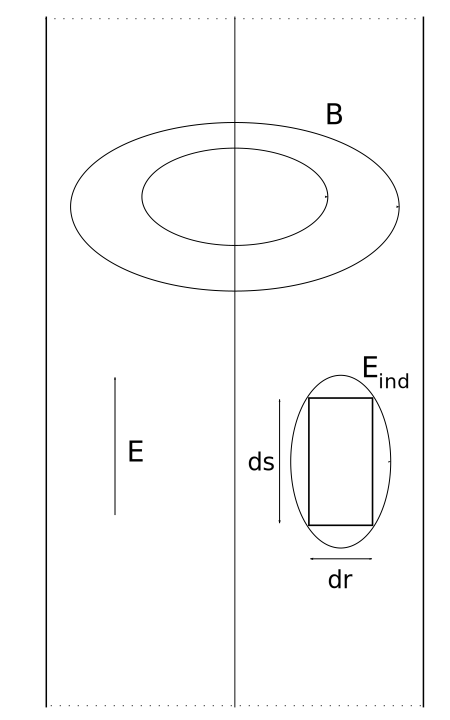
\includegraphics[scale=0.5]{Skineffekt.png}
\end{center}
\caption{Veranschaulichung des Skineffekts} %mehr
\label{pic:skineffekt}
\end{figure}

Zum Verständnis des Effekts betrachten wir ein Flächenelement ds dr im Drahtinneren (vergleiche Abbildung \ref{pic:skineffekt}).
An dem Draht liegt eine Spannung an, welche also ein elektrisches Feld im Draht erzeugt.
Andererseits fließt duch den Draht ein Strom, durch welchen ein magnetische Feld aufgebaut wird.
Da es sich um Wechselstrom handelt, ändert das Magnetfeld ständig seine Richtung und Stärke, wodurch ein elektrisches Wirbelfeld induziert wird.
Auf der der Achse zugewandten Seite ist das induzierte elektrische Feld dem äußerem Feld entgegengerichtet, auf der abgewandten Seite gleichgerichtet.
Das resultierende elektrische Feld und somit auch die Stromdichte muss also von innen nach außen zunehmen.\cite{Gerthsen}

Die genaue Herleitung des Skineffektes ist relativ kompliziert, sie kann in einem Lehrbuch der Elektrodynamik nachgeschlagen werden. % zum beispiel…
Wir wollen hier lediglich eine einfache Herleitung der Eindringtiefe nach \cite{Gerthsen} beschreiben.
Wir starten dabei mit den Maxwellgleichungen, genauer gesagt mit dem Induktionsgesetz von Faraday und dem erweiterten ampèreschen Gesetz:
\begin{align}
\nabla \times \mathbf{E} &= -\frac{\partial \mathbf{B}}{\partial t} \qquad &\mathrm{(Induktionsgesetz\ von\ Faraday)} \\
\nabla \times \mathbf{H} &= \mathbf{j} + \frac{\partial \mathbf{D}}{\partial t} \qquad &\mathrm{(erweitertes\ amp\grave{e}resches\ Gesetz)}
\end{align}
Die elektrische Flussdichte $\mathbf{D}$ hängt mit der elektrischen Feldstärke $\mathbf{E}$ zusammen:
\begin{equation}
\mathbf D = \epsilon_0 \epsilon_r \mathbf{E}
\end{equation}
Da die elektrisches Feldstärke von der Spannung abhängt, stellt auch sie eine Trigonometrische Funktion von $\omega t$ dar, die Ableitung wird somit zu:
\begin{equation}
\mathbf{\dot{D}} = \omega \epsilon_0 \mathbf{E}
\end{equation}\footnote{Warum wir hier das $\epsilon_r$ ignorieren können, habe ich leider nicht herausgefunden.}
Die Stromdichte $\mathbf{j}$ ergibt sich aus der elektrischen Feldstärke und der elektrischen Leitfähigkeit nach dem ohmschen Gesetz zu $\mathbf{j} = \sigma \mathbf E$. Daraus sehen wir, dass für $\omega \ll \frac{\sigma}{\epsilon} \approx 10^{18} s^{-1}$ $\mathbf{\dot{D}}$ vernachlässigbar klein gegenüber $\mathbf{j}$ ist.

Die magnetische Flussdichte $\mathbf B$ hängt analog mit der magnetischen Feldstärke $\mathbf H$ zusammen:
\begin{equation}
\mathbf B = \mu_0 \mu_r \mathbf H
\end{equation} 
woraus folgt:
\begin{equation}
\mathbf{\dot{B}} = \mu_0 \mu_r \mathbf{\dot{H}}
\end{equation} 
Auf der anderen Seite folgt aus obiger Schreibweise des Ohmschen Gesetzes, dass 
\begin{equation}
\rot \mathbf E = \frac{1}{\sigma} \rot \mathbf{j}
\end{equation}
Damit folgt:
\begin{equation}
\rot \mathbf H = \mathbf{j} \qquad
\rot \mathbf E = \frac{1}{\sigma} \rot \mathbf{j} = \mu_0 \mu_r \mathbf{\dot{H}}
\end{equation}
Daraus wird durch Elimination von $H$
\begin{equation}
\rot\rot \mathbf{j} = \sigma \mu_0 \mu_r \frac{\partial \mathbf{j}}{\partial t}
\end{equation}
Die zeitliche Ableitung entspricht einer Multiplikation mit $\omega$, die zweimalige räumliche Ableitung (rot rot) einer zweimaligen Multiplikation mit der reziproken Schichtdicke, auf der der Strom auf $\frac{1}{e}$ abfällt, und wir erhalten:
\begin{equation}
\frac{1}{d^2} \mathbf{j} \approx \omega \rho \mu_r \mu_0 \mathbf{j}
\end{equation}



% wo anders hin verschieben, da auch bei Gleichspannung!?
\subsection{Koronaentladung}
Liegt an einem vergleichsweise dünnem Kabel eine hohe Spannung an, so herrschen in seiner unmittelbaren Nähe sehr hohe elektrische Felder. Sind diese Feldstärken größenordnungsmäßig vergleichbar groß wie die Durchschlagfestigkeit von Luft, so wird die Luft ionisiert, was zu Verlusten führt. Bei Wechselspannung ist dieses Problem besonders groß, da die Scheitelspannung $U_0$ um den Faktor $sqrt{2}$ größer als die Effektivpannung ist, es kommt also im Moment wenn der Scheitelwert erreicht wird auch bei geringeren Effektivspannungen bereits zur Koronaentladung. Dies betrifft insbesondere die 400-kV-Schiene (Scheitelspannung von 566 kV) und macht Übertragungen von mehr als 500 kV per Freileitung fast unmöglich.


\section{Drehstrom}
Beim Dreiphasen-Wechselstrom, auch Drehstrom genannt, hat man drei stromführende Leitungen, an welchen je eine Kosinusförmige Spannung mit gleiche Frequenz, aber jeweils 120\degree Phasenverschiebung anliegt.
Die notwendigkeit eines zusätzlichen Nullleiters entfällt, das die drei Spannungen addiert sich aufheben.
Die Spannung zwischen einer beliebigen Leitung und einen Nullleiter wird als Sternspannung bezeichnet,
die Spannung zwischen zwei beliebigen Spannungen als verkettete Spannung. Es gilt:
\begin{equation}
U_{\mathrm{eff},\:\mathrm{verkettet}} = \sqrt{3} \cdot U_{\mathrm{eff},\:\mathrm{Stern}}
\end{equation}
Die Effekte und Aussagen aus Kapitel \ref{wechsel} gelten ansonsten analog auch für Drehstrom, weshalb wir sie nicht wiederholen wollten.

Während Privathaushalte nahezu ausnahmslos einphasigen Strom verwenden, verwendet man in der Industrie und vor allem in der Stromerzeugung und beim Stromtransport nahezu ausschließlich Dreiphasen-Wechselstrom. Dies bringt mehrere Vorteile\cite{Harrison}:
\begin{itemize}
\item Die durch Drehstrom übertragene Leistung ist zeitlich konstant, wodurch insbesondere Motoren ein zeitlich konstantes Drehmoment haben und somit ruhiger laufen.
\item Bei gegebener Größe hat eine dreiphasige Maschine eine höhere Leistung.
\item Bei gleichem Aufwand kann eine dreiphasiges Stromnetz mehr Leistung übertragen.
\end{itemize}

\section{Elektrische Netze}
\subsection{Leitungen}

\subsubsection{Leitungsbeläge}
Bisher haben wir die Grundlagen der Gleich- beziehungsweise Wechselstromtechnik im allgemeinen kennen gelernt.
Insbesondere bei der Betrachtung von Blindleistungen geht man dabei meist davon aus,
dass ein Verbraucher durch den Einsatz von Spulen oder Kondensatoren Blindleistung erzeugt.
Wir interessieren uns jedoch für die Energienetze und hier kommt ein wichtiger Punkt hinzu:
Auch die Leitungen selbst haben einen Widerstand, eine Kapazität, eine Induktivität, sowie die noch einzuführende Ableitung.
Diese bezeichnet man auf die Länge bezogen als Widerstand-, Kapazitäts-, Induktivitäts- und Ableitungsbeläge und fasst sie unter dem Begriff der Leitungsbeläge zusammen.

Zunächst sei noch die Ableitung eingeführt: Die Ableitungsbeläge beschreiben die Verluste durch unvollständige Isolation des Kabels. Die Ableitung wird in Siemens\footnote{Eine alternative, ältere Bezeichnung für das Siemens ist das Mho (Ohm Rückwerts gelesen) $\mho$ } gemessen, was den Kehrwert der Einheit Ohm darstellt:
\begin{equation}
\mathrm{[S]} = \frac{1}{\Omega} = \frac{A}{V}
\end{equation}
Die Ableitungsbeläge folglich in Siemens pro Meter.
Die Ableitung ist dank moderner Isolationstechnik deutlich geringer als die Ohmschen Verluste.

Bei der Betrachtung der Leitungsbeläge und der daraus folgenden Anforderungen an die Leitungen muss man zwischen drei unterschiedlichen Leitungstypen unterscheiden: Freileitungen, Erdkabel und Unterseekabel %  Begriff richtig?

\subsubsection{Freileitungen}
Der überwiegende Teil der Hochspannungs-Energieverteilung geschieht mit Freileitungen.
Dabei werden nicht isolierte Leiterseile an Isolatoren an etwa 50 Meter hohen und etwa 400 Meter voneinander entfernten Hochspannungsmasten aufgehängt. % Werte für GB
In Deutschland gibt es Freileitungen mit bis zu 380 kV in anderen Ländern auch bis 1000 kV und Anlagen mit bis zu 2 MV sin geplant\cite{Flosdorff}.
Es gibt unterschiedliche Arten und Bauweisen von Freileitungsmasten, auf die wir hier nicht näher eingehen wollen. Wichtig sind für uns lediglich die sich dadurch ergebende Anzahl und Anordnung der Leiterseile, deren Bodenhöhe und Abstand zu einander.

Die Spitze der Masten tragen ein Erdseil, welches die Leiterseile vor Blitzschlag schützen, indem Sie ein Schutzraum bilden. Er wird näherungsweise durch den Zwischenraum zwischen zwei den Boden und das Erdseil tangierenden Kreisen mit doppelter Masthöhe als Radius beschreiben. Die Masten sind derartig gebaut, dass die die Leiterseile sich in diesem Schutzraum befinden. Um bei – bei besonders hohen Spannungen nötige – weiten Travernen den Mast nicht zu hoch bauen zu müssen, kann man durch Verwendung von zwei statt nur einem Erdseil den Schutzraum vergrößern.

Bei den Leiterseilen handelt es sich meist um Verbundseile mit einem Kern aus Stahl, der die mechanische Stabilität gewährleistet, umgeben von Aluminiumleitern. Aluminium hat zwar im Bezug auf das Volumen einen höheren Widerstand als Kupfer, im Bezug auf das Gewicht leitet Aluminium hingegen besser. Ein typisches 650-A-Leiterseil besteht aus 7 Stahl- und 54 Aluminiumadern, die jeweils einen Durchmesser von 3 mm haben.\cite{Harrison}.
Moderne Leiterseile bestehen oft ganz aus einer Aluminiumlegierung und haben dadurch einen höheren Stromtragefähigkeit, einen geringen ohmschen Widerstand und müssen weniger gewartet werden\cite{Harrison}.
%% Skineffekt
Bei höheren Spannungen verwendet man statt einer dicken mehrere dünnere Leiter pro Phase seil in geringem Abstand. Dadurch sind die Randfeldstärken\footnote{Die Randfeldstärke darf zur Vermeidung von Koronaentladung nicht größer als 17 kV/cm werden.\cite{Flosdorff}} und die Induktivität geringer und durch die bessere Kühlung aufgrund der größeren Oberfläche kann ein größerer Strom geführt werden. Man spricht hier von Bündelleitern.
Seit einigen Jahren stattet man vor allem die Erdseile, aber auch die Leiterseile mit Lichtwellenleitern zur Datenübertragung aus. Diese dienten zunächst der innerbetrieblichen Fernüberwachung- und -steuerung, wird heute jedoch vor allem auch für privat genutzte Telefonnetze verwendet.\cite{Flosdorff}
% Durchhang, entfernung, Last, Wetter, etc. ?

In Abbildung \ref{fehlt} ist ein Ersatzschaltbild für eine Einphasige Leitung mit den Leitungsbelägen gezeichnet. Dabei ist R der serielle Widerstand, L die serielle Induktivität, C die Parallele Kapazität und $R_0$ der Ableitungswiederstand. Für die genaue Betrachtung muss man sich dieses infinitesimal Klein, unendlich oft hintereinander geschaltet vorstellen, für kurze Leitungen (unter 100 km Länge), kann man es jedoch näherungsweise auf eine derartige Schaltung reduzieren.
Typische Werte für den Widerstand, die Induktivität und Kapazität findet man in Tabelle \ref{fehlt}. Der Wert für die Ableitungsbelag hängt stark von äußeren Faktoren, wie den Umgebungsbedingungen und dem Verschmutzungsgrad der Isolatoren ab. Ein typische Wert ist $200\,M\Omega m^{-1}$.\cite{Harrison} Die Ableitungsverluste sind also meist deutlich geringer als die seriellen ohmschen Verluste, weshalb man sie in den meisten Betrachtungen ignorieren kann.
Wie wir sehen ist eine Freileitung weitgehend induktiv. Die Induktivität lässt sich für eine einphasige Leitung wie folgt berechnen:
\begin{equation}
L = \frac{\mu}{\pi} \cdot \left[ \frac{1}{4} + \ln\left(\frac{d}{rs}\right) \right]
\end{equation}
Dabei ist $r$ der Radius des Leiters und $d$ der Abstand der Leiters zur nächsten Erdpotential - also gewöhnlich das Leiterseil des Nullleiters. Für Luft wird daraus:
\begin{equation}
L = 4 \cdot 10^{-7} \cdot \left[ \frac{1}{4} + \ln\left(\frac{d}{rs}\right) \right]
\end{equation}
Hat man eine dreiphasen-Übertragung, so hängt die Induktivität von der Anordnung der Leiter ab. Für eine symmetrische Anordnung der Leiter gilt:
\begin{equation}
L = \frac{\mu}{2\pi} \cdot \left[ \frac{1}{4} + \ln\left(\frac{d}{rs}\right) \right]
\end{equation}
vorausgesetzt wird dabei das die Höhe über der Erde $h\gg d$ ist, ansonsten muss diese mit berücksichtigt werden.
Sind die Leiter nicht symmetrisch angeordnet, haben sie eine unterschiedliche Induktivität und es kommt dadurch zu einem unterschiedlichem Stromfluss.
Um dies zu vermeiden, kann man die Leiterpositionen an Zwischenstationen zyklisch vertauschen. Dann gilt auch obige Formel mit $d_eq = \sqrt[3]{d_{12}+d_{23}+d_{31}}$ statt $d$.

%% Vereinfachung
%% Formel für Last

\subsubsection{Kabel}
In urbanen Gegenden sowie in Gegenden mit besonders erhaltenswerten Landschaften, setzt man statt Freileitungen auf unter der Erde verlegt Kabel. Die Leiter sind in der Regel aus Kupfer oder Aluminium und mit Ölimpregniertem Ölband oder neuer mit flüssigkeitsimprägniertem Propylen/Papier-Laminat isoliert. 
Letztere haben eine um 67\% niedrigere dielektrische Verluste und eine 20\% niedrigere Permittivität und somit Kapazität.\cite{Harrison} Dadurch lässt sich mehr Leistung übertragen und es muss weniger Blindleistung bereitgestellt werden.
% höhere Kosten, nidrigere Zuverlässigkeit
Das Ersatzschaltbild sieht wie das der Freileitung aus, nur das man zwei Parallel geschaltete Ableitungswiederstände betrachtet.
$R_0$ ist der Isolationswiederstand, während $R_d$ die dielektrischen Verluste beschreibt. Das sind Verluste die durch Polarisationseffekte im Dielektrikum der Kapazität entstehen.
Typische Werte für ein einphasiges Kupferkabel findet man in Tabelle \ref{fehlt}.
Wie wir mit den Werten feststellen können, ist bei Kabeln die Kapazität überwiegend,
besonders stark ist dies bei Unterseekabeln ausgeprägt. % überprüfen, warum?, Werte
Dazu kommt, dass bei Unterseekabeln die Blindleistungskompensation nur schwer möglich ist.
Die hohen Kapazitäten erfordern hohe Ströme zum Laden der Kapazität (Ladeströme), welche durch den gesamten zur Verfügung gestellten Strom aufgebracht werden müssen. Dies reduziert die übertragbare Leistung und führt ab einer gewissen Länge dazu, dass der maximal übertragbare Strom als Ladekapazität benötigt wird. % versteh ich selbst nur halb...
Für ein 400-kV-Kabel wie in Tabelle \ref{fehlt} liegt diese Länge bei 43,6 km.
Daher werden bei längeren Kabeln alle paar Kilometer % wieviel genau, besser formulieren…
Induktivitäten angeschlossen um die Blindleistung zu kompensieren.


\section{Vor- und Nachteile der HGÜ gegenüber DHÜ}

\section*{bla}
\begin{circuit}{2}
\R1 {$1 \Omega$} h
\- 8 r
\C1 C d
\- 4 v
\nl\R1 {L} d 
\nl\- 10 v
\end{circuit}

\begin{circuit}{0}
\npn1 {?} B l
\frompin npn1C
\- 1 u
\nl\A1 {$I_C$} u
\atpin npn1B
\- 1 l
\R1 {510 kohm} l
\end{circuit}


\bibliography{lit}{}
\bibliographystyle{plain}

\end{document}
